\documentclass[a4paper,10pt]{article}
\usepackage[margin=1in]{geometry}{}
\usepackage[utf8]{inputenc}
\usepackage[T1]{fontenc}
\usepackage{graphicx}
\usepackage{xcolor}
\usepackage{hyperref}
\usepackage{enumitem}
\usepackage{parskip}
\usepackage{fontawesome5}
\usepackage{pdfpages} % Added for including PDF certificates
\usepackage[most]{tcolorbox}
\hypersetup{
  colorlinks=true,
  urlcolor=blue!60!black, % dark blue for links
  linkcolor=black
}

\definecolor{modernblue}{RGB}{36,113,163}

\newcommand{\cvsection}[1]{%
  \vspace{0.8em}
  \noindent\colorbox{modernblue!10}{\parbox{\dimexpr\linewidth-2\fboxsep}{\textbf{\large\color{modernblue} #1}}}
  \vspace{0.2em}
}

\usepackage{lmodern}
\renewcommand{\familydefault}{\sfdefault}

\begin{document}
\pagestyle{empty}

\begin{tcolorbox}[colback=modernblue!5!white, colframe=modernblue, boxrule=0.5mm, arc=2mm, left=2mm, right=2mm, top=1mm, bottom=1mm, width=\textwidth, enlarge left by=0mm, enlarge right by=0mm]
    \begin{center}
        {\LARGE \textbf{Mateo Nicolas Torres Vara}}\\[1em]
        \renewcommand{\arraystretch}{1.2}
        \begin{tabular}{@{} l l @{}}
            \faIcon{phone}~+51 987803624 &
            \faIcon{envelope}~\href{mailto:torresvaramateo@gmail.com}{\textbf{torresvaramateo@gmail.com}} \\
            \faIcon{github}~\href{https://github.com/MateoTVara}{\textbf{github.com/MateoTVara}} &
            \faIcon{linkedin}~\href{https://www.linkedin.com/in/mateo-torres-vara-75ba57292/}{\textbf{mateo-torres-vara-75ba57292}}
        \end{tabular}
    \end{center}
\end{tcolorbox}

\vspace{0.5cm}

\cvsection{Perfil}
\\
Estudiante de Ingeniería de Sistemas en la Universidad Tecnológica del Perú, actualmente cursando el octavo ciclo. Técnico en Desarrollo de Sistemas de Información por el Instituto IDAT (2022-2024). Apasionado por el desarrollo web, con sólidos conocimientos en lenguajes de programación, frameworks y bases de datos. Nivel de inglés B2 certificado.

\cvsection{Educación}
\begin{itemize}[leftmargin=0.7cm, label=\faIcon{graduation-cap}]
    \item \textbf{Ingeniería de Sistemas} \\
    Universidad Tecnológica del Perú \\
    Ciclo 8 en curso
    \item \textbf{Técnico en Desarrollo de Sistemas de Información} \\
    Instituto IDAT (2022 -- 2024)
\end{itemize}

\cvsection{Habilidades Técnicas}
\begin{tcolorbox}[colback=gray!5!white, colframe=gray!50!black, boxrule=0.2mm, arc=1mm, left=1mm, right=1mm, top=1mm, bottom=1mm, width=\textwidth]
\textbf{Lenguajes de programación:}
\begin{itemize}[leftmargin=0.7cm, label=\faIcon{code}]
    \item JavaScript \& Node, Python, Java
\end{itemize}
\textbf{Frameworks:}
\begin{itemize}[leftmargin=0.7cm, label=\faIcon{cogs}]
    \item Django, Spring Boot, React
\end{itemize}
\textbf{Herramientas y tecnologías:}
\begin{itemize}[leftmargin=0.7cm, label=\faIcon{tools}]
    \item Git, GitHub, Postman
\end{itemize}
\textbf{Otros lenguajes:}
\begin{itemize}[leftmargin=0.7cm, label=\faIcon{file-alt}]
    \item SQL, CSS, HTML, LaTeX, Markdown
\end{itemize}
\end{tcolorbox}

\cvsection{Certificaciones}
\begin{itemize}[leftmargin=0.7cm, label=\faIcon{certificate}]
    \item NDG Linux Essentials course in the Cisco Networking Academy
    \item PCAP: Programming Essentials in Python
    \item First Certificate in English (B2)
\end{itemize}

\cvsection{Idiomas}
\begin{itemize}[leftmargin=0.7cm, label=\faIcon{language}]
    \item Español (nativo)
    \item Inglés (B2 certificado)
\end{itemize}

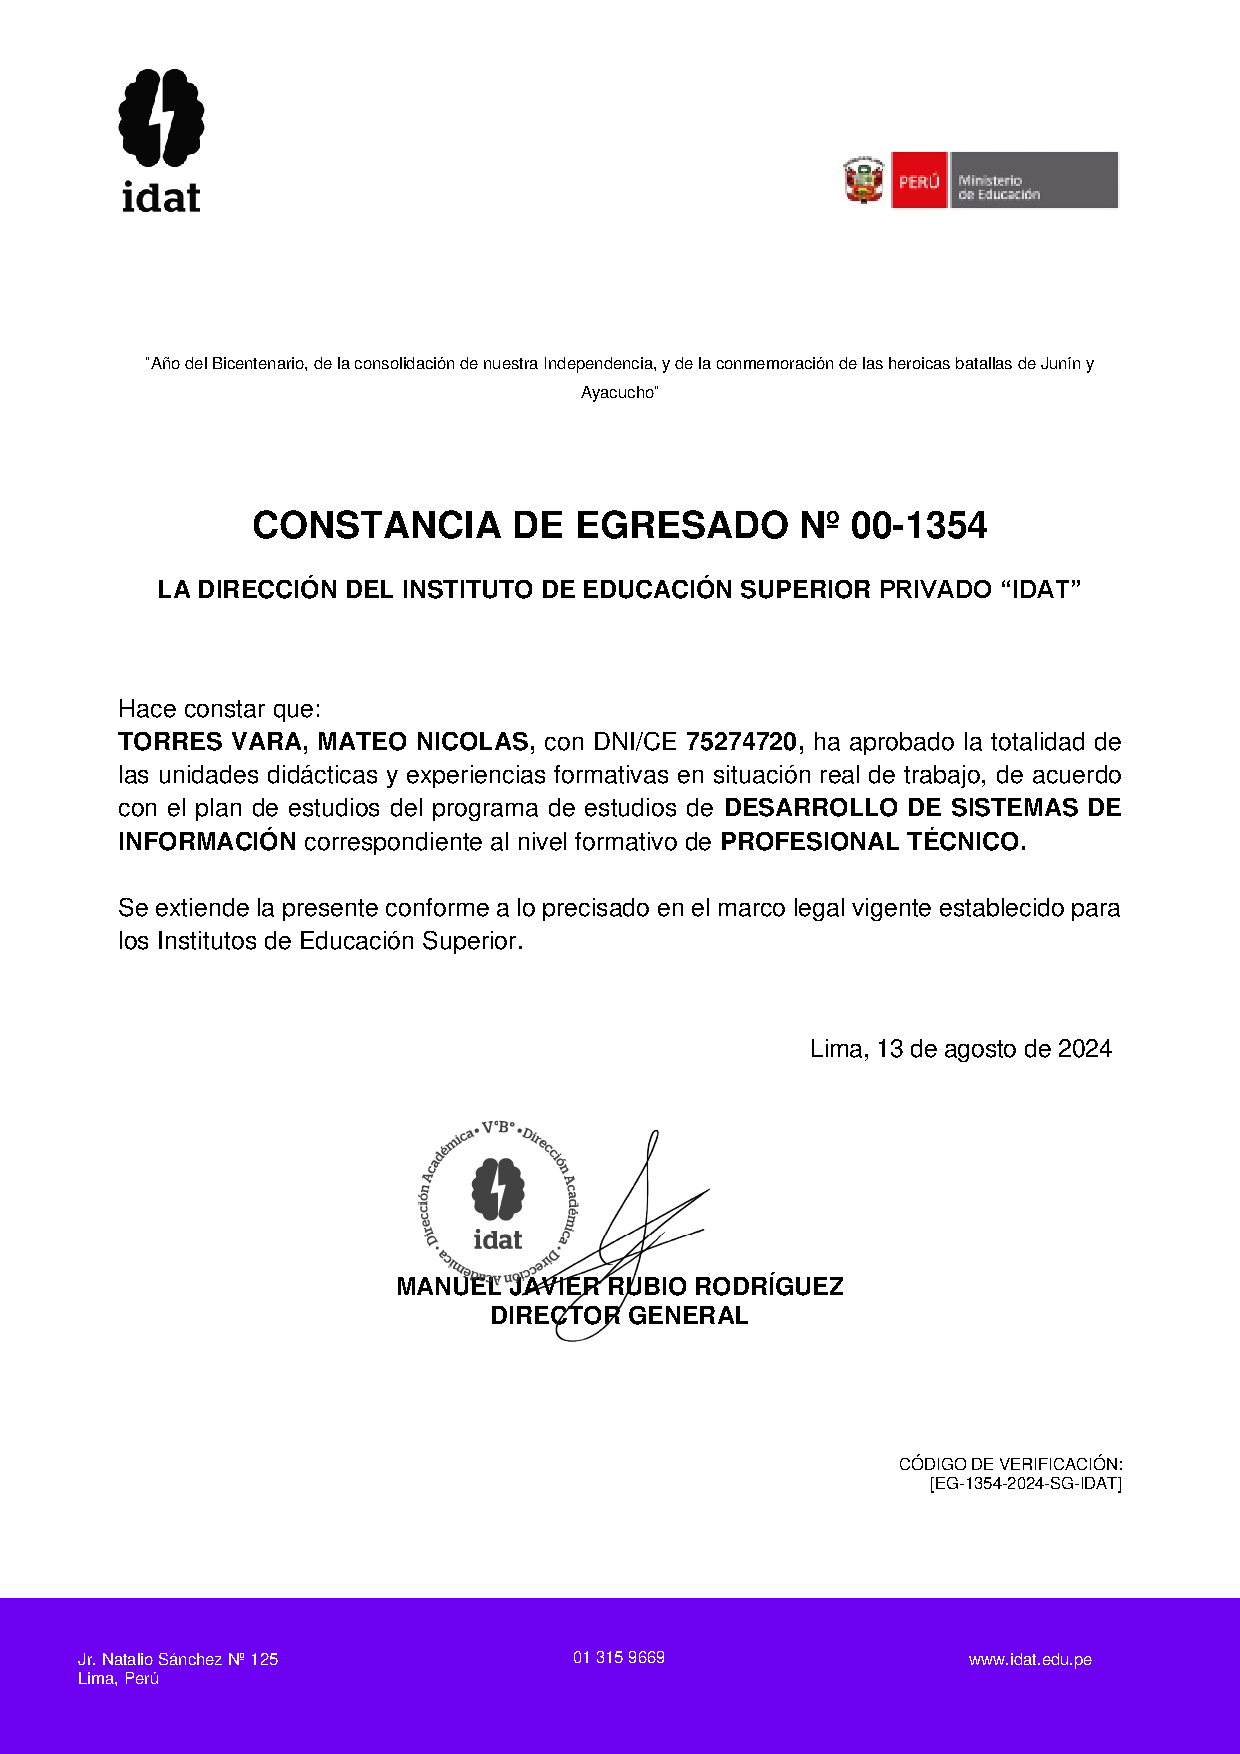
\includepdf[pages=-]{../assets/constancia_idat.pdf}

\includepdf[pages=-,landscape,fitpaper=true]{../assets/linux_essentials.pdf}
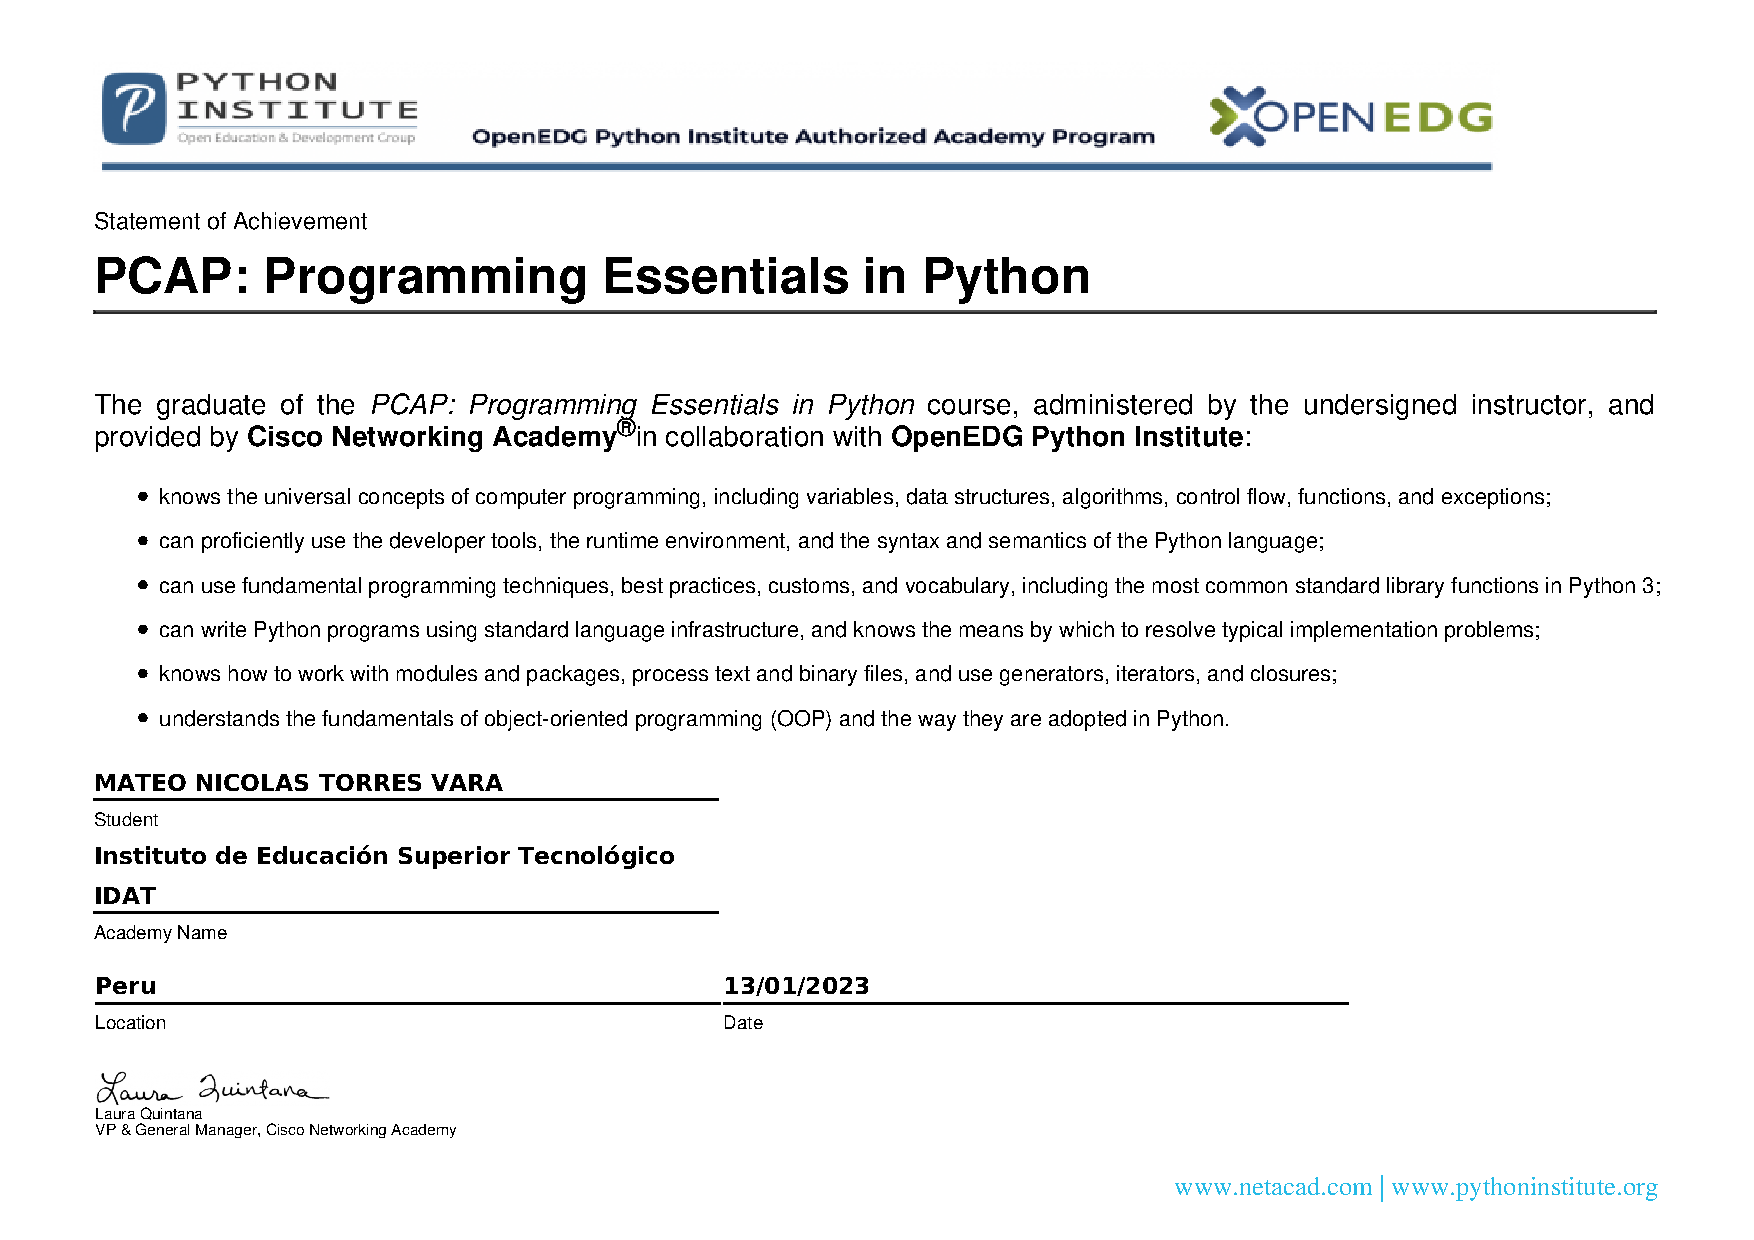
\includepdf[pages=-,landscape,fitpaper=true]{../assets/programming_essentials_in_python.pdf}
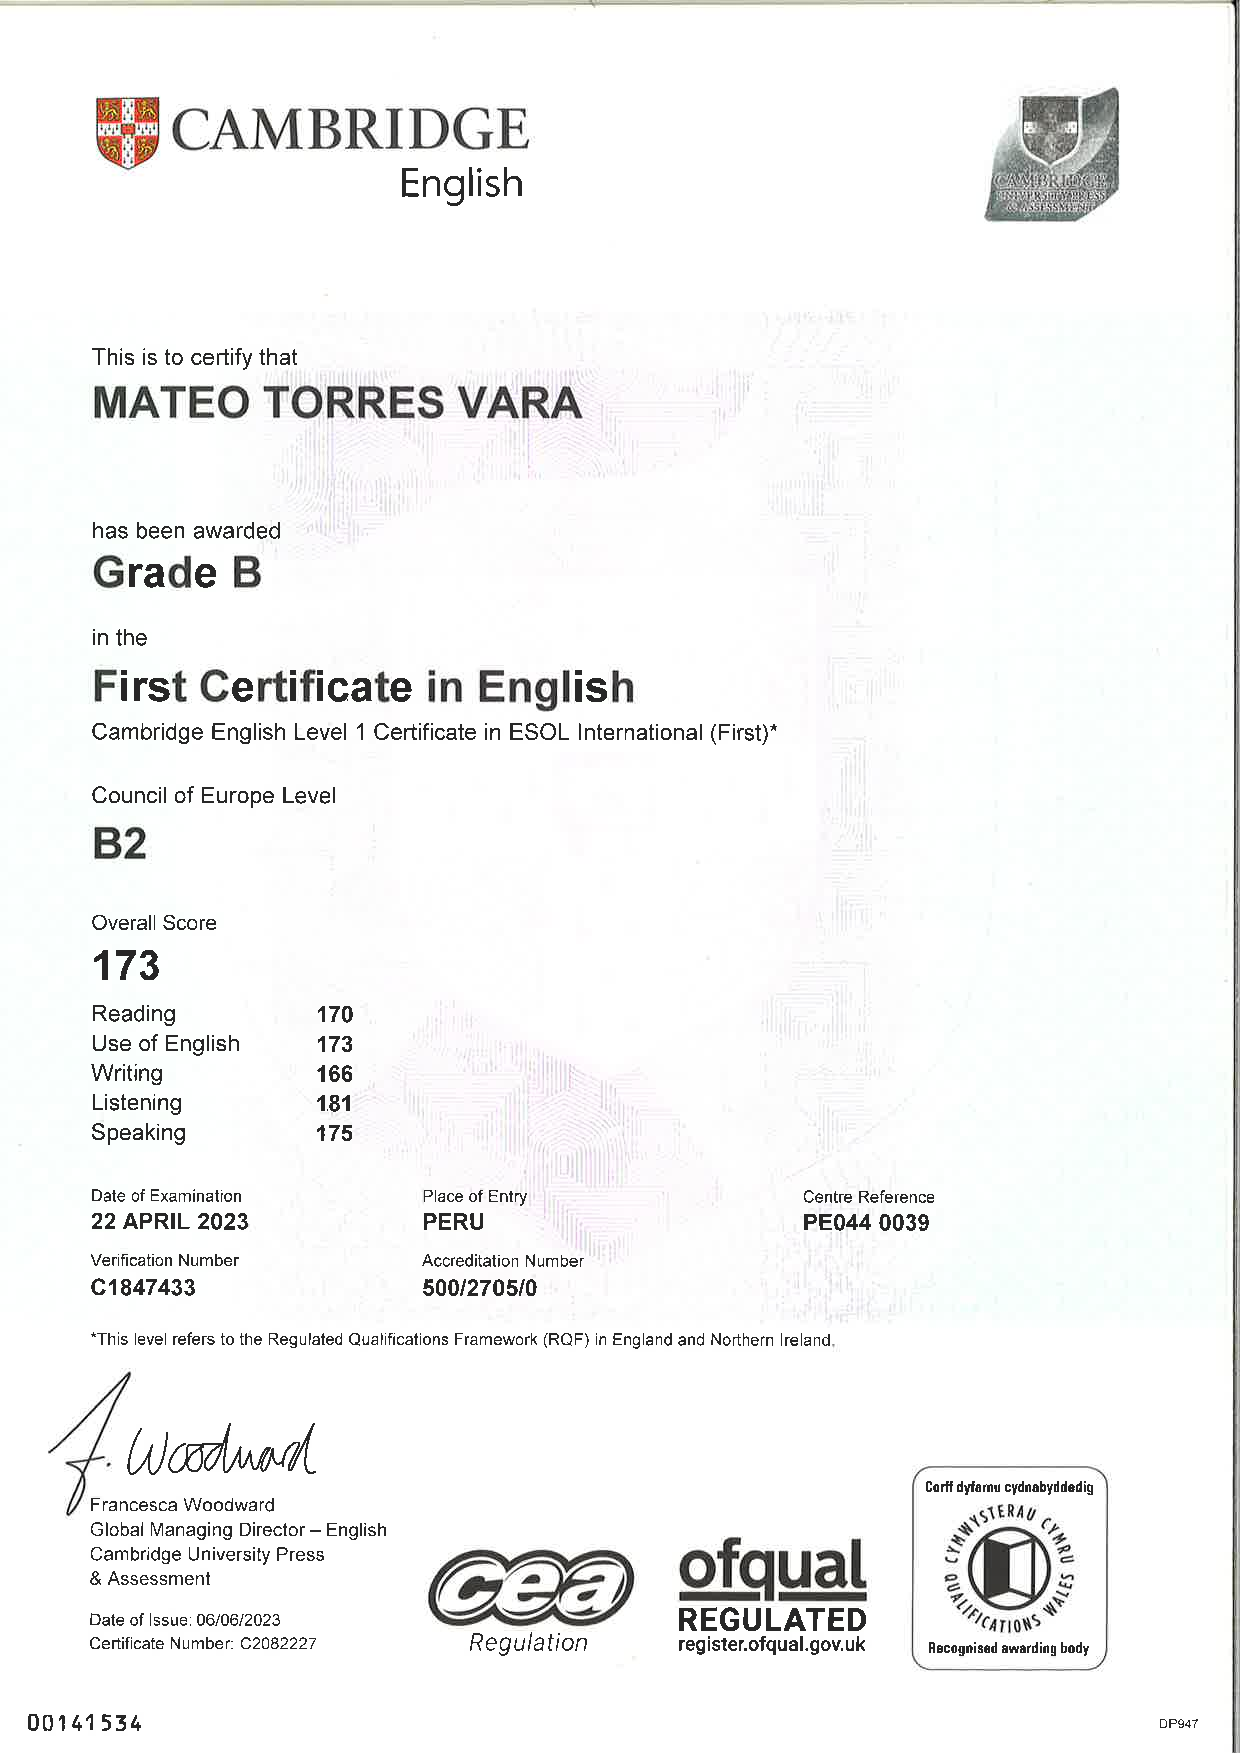
\includepdf[pages=-]{../assets/first_certificate_in_english.pdf}

\end{document}